\section{Literature Review}\label{sec:lit_rev}
Natural Language Processing (NLP) has come a long way from the era of batch processing and punch cards where a sentence analysis query used to take almost seven minutes to the era of search engines like Google and Bing where millions of web pages are crawled within seconds to produce the best results \cite{Cambria2014}. NLP is a way for computers to perform natural language related tasks like information extraction (like POS tagging, Named Entity Extraction) or language generation and summarisation (like machine translation, dialogue systems) \cite{Young2018}.

% There are different types of tasks in NLP guiding the research in this domain ranging from lower level problems like NER and POS tagging to higher level problems like machine translation and question answering. 
In the next \cref{sec:tasks}, we briefly discuss the various tasks of NLP on different levels. To solve these tasks, there are various methods in the literature which we broadly divide into two categories; Knowledge Engineering (\cref{sec:ke}) and Representation Learning (or in common words, deep learning \cref{sec:dl}). Earlier, knowledge engineering approaches were use to solve NLP tasks. But problem with these methods is that they rely on domain expertise for engineering the knowledge from data. With the development and success of deep learning methods in vision tasks, deep learning has been employed for NLP tasks as well and has been successful as well. The benefit of these methods is that they do not need any special knowledge engineering as they automatically learn features modelling the data during their training phase. This learning is iteratively updated in various steps during training.
% The main difference between two is that the former requires a lot of feature engineering whereas the later automates the process of feature extraction using dense representation of text. 
% In the final \cref{sec:initial_work}, we will take a real world example using the compliance data from Oil and Gas industry and evaluate these methods.

% The techniques present in literature for solving these tasks. We will briefly discuss about how the fields of industry and academia differ in taking to approaches to the solution for these tasks.

% Solving these NLP tasks were a real hassle for a long time. They required an extensive need of domain expertise in order to derive some knowledge that will suit for a given problem. But with the advancement of deep learning in the field of NLP we have got new solutions that are not specific to the domain of the problem. Same method can be applied to different problems from different domains with very little fine tuning with respect to domain specific data.

% The breakthroughs in academic research take a long time to be implemented in the industry. This is due to problem of available labelled data-set for training the 

% Here we can broadly divide the problem solving approaches into two categories: knowledge engineering and deep learning. 


% \section{Background on NLP}
\subsection{Tasks}\label{sec:tasks}
NLP research is mostly driven by the basic question, how do humans understand the natural language and how can we make the machines do the same? In the research, understanding the natural language for machines differs from lower level problems of extracting information from the text like named entity or relation extraction to higher level problems like machine translation or question answering. In this section we will discuss about the different kind of tasks involved in NLP dividing them into three broad categories:

\begin{enumerate}
    \item Extraction
    \item Generation
    \item Summarisation
\end{enumerate}

\subsubsection{Extraction}
Knowledge Extraction is a sub field of NLP that deals with the automated extraction of structured knowledge from unstructured sources. These are the few examples of the tasks that can be treated as knowledge extraction.

\paragraph{Named Entity Recognition}
Named Entity Recognition is the a sub task of Knowledge Extraction that deals with identifying the various entities in a piece of text such as person, location, organization and date. It has various use cases, like automating hiring process or optimizing the search engine algorithms. One of the main approach is to use BIO notation (B for beginning, I for inside and O for non-entity tokens.) For example, in the sentence \textit{`Boris Johnson won the UK general elections'} the entities can be marked as $[Boris]_{B-PER}$ $[Johnson]_{I-PER}$ $[won]_{O}$ $[the]_{O}$ $[UK]_{LOC}$ $[general]_{O}$ $[elections]_{O}$. PER represents person, LOC represents location and O is the non-entity tokens.

There are various open source libraries for NER such as spaCy which uses hand crafted features (not published) and StanfordNLP which uses a combination of hand crafted features and deep learning for the same task. One of the most popular benchmark for NER is CoNLL 2003 \cite{sang2003introduction} consisting text from news wires like Reuters dataset tagged in four different categories (PER, LOC, ORG, MISC). The state-of-the-arts in literature for NER right now are mostly based on the transformers architecture which we will discuss is \cref{sec:transformers}

% NER SRL Chunking sequence tagging
% Named Entity Recognition deals with 

\paragraph{Parts-of-Speech Tagging}
deals with the marking of parts of speech of a word in the text corpus. The category of words having similar grammatical properties can be termed as parts-of-speech. Some of the common parts-of-speech in English language are noun, pronoun, adjective, preposition, verb, adverb etc. NLTK is one of the most common open-sourced library used for POS tagging. A example of POS tagging in NLTK for the sentence \textit{`And now for something completely different'} can be \textit{[('And', 'CC'), ('now', 'RB'), ('for', 'IN'), ('something', 'NN'),
('completely', 'RB'), ('different', 'JJ')]}. Here CC is coordinating conjunction, RB is used for adverbs, IN is a preposition, NN is noun and JJ is adjective \footnote{Example taken from \url{https://www.nltk.org/}}.

The popular benchmarks for POS tagging are Penn Treebank \cite{marcus1993building} and Universal Dependencies \cite{silveira14gold}. Penn Treebank portion of Wall Street Journal (WSJ) consists of 45 different POS tags whereas Universal Dependencies consists of more than 100 treebanks from 60 different languages. The current state-of-the-arts for POS tagging are mostly based on LSTM and BERT.

\paragraph{Natural Language Inference}
For a given piece of text or premise, finding that whether some `hypothesis' about that text is true or not is called natural language inference. If a hypothesis is true then it is known as `entailment', if it is false then `contradiction' and for undetermined `neutral'. For example, lets have a look at the \cref{tab:nli} \footnote{Example taken from \url{https://nlpprogress.com/}}.

\begin{table}[h!]
  \begin{center}
    \caption{NLI Example}
    \label{tab:nli}
    \begin{tabular}{l|c|r} % <-- Alignments: 1st column left, 2nd middle and 3rd right, with vertical lines in between
      \textbf{Premise} & \textbf{Label} & \textbf{Hypothesis}\\
      \hline
      A man inspects the uniform of a & contradiction & The man is sleeping.\\
      figure in some East Asian country. &  & 
    \end{tabular}
  \end{center}
\end{table}

The two most common corpus for NLI are Multi-Genre Natural Language Inference (Multi-NLI) \cite{williams2017broad} and Stanford Natural Language Inference (SNLI) \cite{bowman2015large}. Both of them contain around 500k labelled hypothesis/premise pairs. Current state of the arts are based on the slight modification of BERT architecture.

\paragraph{Relation Extraction}
The task of identifying semantic relationships between entities of text is known as relation extraction. Usually the relations are defined between two or more entities like person, location or organisation and fall under various pre-defined semantic categories.

There are lots of public datasets available for relation extraction and all of them define their own category of relations that need to be extracted from the text. Few examples are; Capturing discriminative attributes (SemEval 2018 Task 10) \cite{krebs2018semeval} where users are asked to identify if a given attribute can help in discrimination between two concepts. Few-Shot Relation Classifier (FewRel) \cite{han2018fewrel} consisting of 70k sentences with 100 different kinds of relation annotated by crowd-sourcing on wikipedia corpus. New York Times corpus \cite{riedel2010modeling} containing entities extracted from NYT corpus and linked to the freebase knowledge base. 
% There are different types of state-of-the-arts based on hand crafted features as well machine/deep learning algorithms to achieve good results on these datasets.

% \paragraph{Template Filling} The approach of efficient extraction and representation of 

% \paragraph{Semantic Role Labelling}


% \paragraph{Dependency Parsing}

\subsubsection{Generation}
Natural Language Generation (NLG) can be termed as the sub-field of NLP which deals with the generation of natural language given some structured or unstructured information. Machine Translation and Data Augmentation can be few examples of NLG.

\paragraph{Machine Translation}
Machine Translation has been one of the most popular problems in NLP. It deals with the translation of text from one natural language to another, for example, translating English text to Hindi or vice-versa. A snippet from Google translate performing MT is shown in fig. \ref{fig:mt_example} \footnote{\url{https://translate.google.com/}}.

\begin{figure}
    \centering
    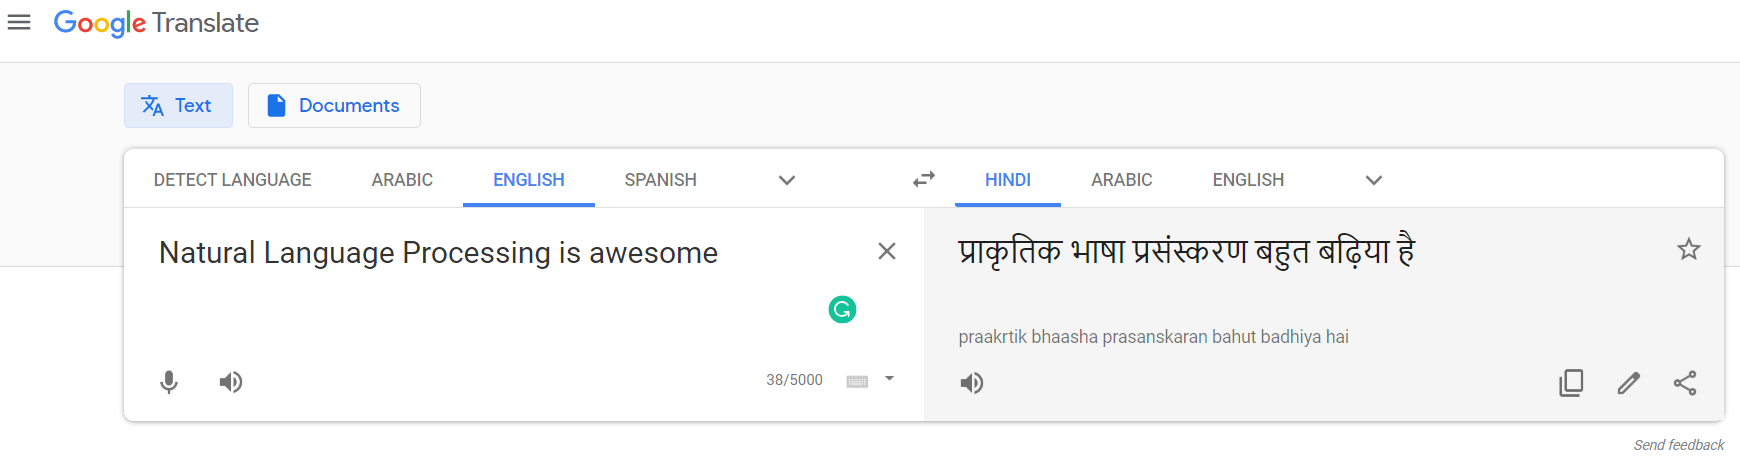
\includegraphics[width=\textwidth]{images/mt.png}
    \caption{An Example of Machine Translation}
    \label{fig:mt_example}
\end{figure}

The MT models are evaluated on the method called BLEU score which is used as the higher the better. Some of the common public datasets availabel are WMT 2014 EN-DE and WMT 2014 EN-FR \cite{bojar-EtAl:2014:W14-33} which contains many english-german and english-french pair of sentences. The current state-of-the-arts are based on mainly transformers and some attention based LSTMs.

\paragraph{Data Augmentation}
With the popularity of Deep Learning based NLP, there has been a huge requirement of training data for building the models. Collecting the labelled data is sometime very costly and take a lot of resource in terms of time and money. 

The alternative way of getting more data is to generate a huge corpus of data by tweaking the using the small amount of training data available in some fashion. This technique is known as data augmentation. The way of tweaking differs from problem to problem. There are different ways of data augmentation like unsupervised back translation with consistency training \cite{Xie2019} or contextualized word replacement \cite{kobayashi2018contextual}.

\subsubsection{Summarisation}
The third category of NLP tasks is termed as the problem of summarisation. Given a piece of text, how can we summarize the information it posses in simpler and/or structured manner. 

\paragraph{Text Classification}
Classifying a piece of text/document into some pre-defined categories can be termed as the task of text classification. Text classification is mainly used in applications like sentiment analysis and/or topic and document classification. 

For example, in sentiment analysis we try to identify the sentiment or polarity of a sentence based on its content. Given a review about a product on Amazon and identifying if the customer who wrote the review is positive or negative about the product's quality. Some of the common examples for topic classification can be identifying the domain (political, religious or technological) of a news article based on its content.

Some popular datasets for sentiment analysis are; imdb movie reviews which contains 50,000 reviews of different movies from imdb website labelled into positive and negative classes. They also contain a numeric value from 1 to 10, 1 being the lowest rating and 10 being the highest rating. The current state-of-the-art is XLNet based on the transformer architecture for this \cite{yang2019xlnet} dataset.

Another famous dataset for text classification is Dbpedia dataset which consist of 5.6M labelled texts from the 14 non-overlapping topics of wikipedia. BERT \cite{devlin2018bert} is the current best performing algorithm with only 0.64 error rate on this dataset.

\paragraph{Question Answering}
Question Answering is a token-level task of NLP where given a piece of information with some question related to it, the system needs to generate an acceptable answer for it. One of the most famous dataset for this task is Stanford's Question Answering Dataset (or SQuAD) which consists of different questions asked by users of wikipedia related to some wikipedia article. The answer to this question is a segment from the same article only. The current state-of-the-arts for this datasets are the ensemble models based on different versions of BERT. An updated leaderboard for this dataset can be found on their website \footnote{\url{https://rajpurkar.github.io/SQuAD-explorer/}}.

% \paragraph{Aspect-Based Sentiment Analysis}

% \paragraph{Summary Generation}
% Chat-bots in NLP are very popular in today's world. They can interact with the users in a very humane manner and are very efficient. Suppose, a company has to interact with their customers on the website on the daily basis. One way to answer the queries of these customers will be have support assistants hired to answer these queries as the part of their job. But this can be very expensive. On the other hand, the company can use an automated software to do the same job if 

\subsection{Knowledge Engineering}\label{sec:ke}
Initially, the solutions for NLP problems were all based on a common approach of identifying better features to represent the text data. These features are identified based on the domain expertise and are very specific to the problem they are applied in. This category of techniques can be classified as the techniques which requires a lot of domain knowledge in order to achieve good results. They don't need a lot of training data in order to gain good performance but the performance gets saturated after some amount of data, i.e., the performance doesn't increase with the increase in training data. We group these methods into two categories:

\begin{enumerate}
    % \item Rule Based
    \item Case Based Reasoning
    \item Machine Learning
\end{enumerate}

% \subsubsection{Rule Based}
% The techniques which requires a pre-defined set of rules to identify the matches and solve the problem.

% \paragraph{Syntax driven} It takes a syntax driven approach to semantic 

% is the approach where syntax

% \paragraph{Lexicon approach} requires a set of dictionary/lexicon defined in order to identify 

% \paragraph{Ontology based}

% \paragraph{Linguistic Features}\label{sec:ling_ftrs}
% A sentence can be processed to extract parts of speech, noun chunks, and entities. Some of the features that can be generated afterwards are as follows:

% \begin{enumerate}
%     \item word length: number of tokens in sentence.
%     \item word length 2: number of words in sentences with stopwords removed.
%     \item has modal: indicates if the sentence contains a modal.
%     \item num of modals: number of modals in sentence.
%     \item modal position: average position of modal verbs in a sentence (-1 if none).
%     \item num of entities: number of named entities in sentence.
%     \item m trigger word: checks if the sentence contains any mandatory term (true/false).
%     \item m trigger position: average position of mandatory terms in sentence ([0.0,1.0] interval and -1 if none).
%     \item n trigger word: checks if the sentence contains any non-mandatory term (true/false).
%     \item n trigger position: average position of non-mandatory terms in sentence ([0.0,1.0] interval and -1 if none).
% \end{enumerate}


\subsubsection{Case Based Reasoning}
Case Based Reasoning is a sub-field of Artificial Intelligence which solves the problems on the basis of modelling real word intuition that similar problem have similar solutions. When we see a new problem in our real life, we try to map it to our previous experience of similar problems and solve it taking similar approach. In CBR as well, we retrieve the problems similar to the new one and use the similar kind of approach to solve it using the solutions stored in knowledge base (KB). In the KB, we store these cases in a pair of problem and solution. A CBR cycle generally have 4 steps as defined in \cite{aamodt1994case}. Fig. \ref{fig:cbr_4r} shows the 4Rs of a CBR cycle.

\begin{enumerate}
    \item RETRIEVE the cases similar to the new problem.
    \item REUSE the information or solution for similar cases to solve the new one.
    \item REVISE the new proposed solution.
    \item RETAIN the useful information of new case in the KB for future use.
\end{enumerate}

\begin{figure}
    \centering
    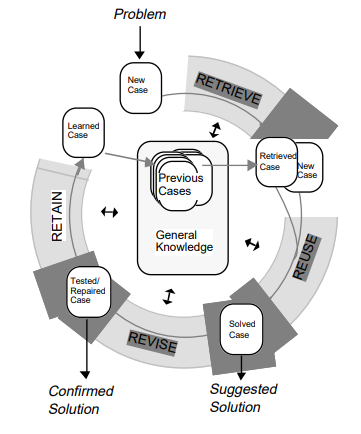
\includegraphics[width=0.45\textwidth]{images/cbr_4r.png}
    \caption{4Rs of a CBR Cycle \cite{aamodt1994case}}
    \label{fig:cbr_4r}
\end{figure}

\paragraph{k-Nearest Neighbours (k-NN)} One of the most common CBR algorithm is k-Nearest Neighbour which computes the distance between the new case and all other previous cases. Then the k cases with the minimum distance are selected as the similar cases and there solution is used to make decision for the new case's solution. k-NN uses the euclidean distance to measure distance between two cases. The distance between two cases $c_{i}$ and $c_{j}$ is given in \cref{eq:knn}

\begin{equation}
    \label{eq:knn}
        Dist(c_{i}, c_{j}) = \sqrt{\sum_{v=1}^{n} (c_{iv}-c_{jv})_{2}}
\end{equation}

where v is the dimension of problem in the case. This technique is also referred as lazy learning sometimes as it makes observation on the previous knowledge every time a new query is given rather than trying to learn a general model for knowledge base in training and using that model to answer a query when asked.

\paragraph{Textual Case-Baed Reasoning (TCBR)}
TCBR is a bit different from general CBR in terms of representation of problem and solution of the cases, altough the 4Rs of a CBR cycle holds true here as well. In TCBR, some or whole part of the previous cases are stored in textual form and we aim to solve the problem for new cases with the help of these textual knowledge sources in automated way \cite{weber2005textual}. The cases are stored in two sets namely, problem set and solution set. In TCBR, the focus is on defining a good representation of these sets and then finding a way to evaluate these representations.

\paragraph{Text Representation}
Representing cases in text CBR is a trivial task as there is no standard representation defined that can work for every problem. But one of the most commonly used representation is using bag of words \cite{10.5555/646268.684025}. In this representation, a sentence is is broken into tokens which are essentially the words of the sentence and their appearance is different manner is used as the features. One of the drawback of using this technique is that we loose the sequence information as it is lost during the tokenisation process.

Another common way of representing texts is by grouping them into attribute-value pairs to generate feature vectors, where attributes are decided based on the domain and values are the pieces of text from the case base. This approach works for maximum cases but the attributes differ from problem to problem as they are domain specific. An example of attribute-value pair can be a case storing the information of a student with attributes such as \textit{Student Name - Ashish Upadhyay} and \textit{School - Computing Science and Digital Media}.

There are other examples of case representation as well, like used in popular CBR framework jCOLIBRI where cases are stored in tree structure where each case is treated as an individual capable of containing other individuals and thus forming the tree structure.

\paragraph{Evaluation}
After the representation of text cases is done, we need to evaluate it by measuring the similarity or alignment between cases problem and solution set. A good representation will provide much better alignment between cases than a bad representation.

Two most common ways of measuring the similarity can be local alignment and global alignment \cite{raghunandan2008evaluation}. The local alignment measure uses the alignment of each case with its neighbourhood and then aggregates the values for all cases to find the alignment for whole case base whereas the global method measures the alignment value for whole case base as one single entity.

\subsubsection{Machine Learning}
Machine Learning is another subset of Artificial Intelligence which learns a general distribution of the previous experience by using the training data and then uses the learned distribution to predict the answer a new problem. In Machine Learning, we mostly use sparse representation of the problems of a case and use statistical algorithms to learn the general distribution of training set.

The difference of machine learning approach from case-based approach is that machine learning, the distribution is learned during the training process and that learning is used to answer a query during test or deployment phase whereas in case-based reasoning, the case-base is searched to retrieve the similar cases every time a query is asked in order to answer it.

Some of the representations and learning algorithms used in machine learning are briefly discussed here. Term Frequency (TF), Term Frequency-Inverse Document Frequency (TFIDF) and Linguistic Features are some of the most common feature representations, whereas Support Vector Machines, Random Forest and Naive Bayes are some of the commonly used learning algorithms.

\paragraph{Term Frequency Vectors}
This feature vector is used to represent a document by assembling a vector of the frequency of the terms contained in the document. Here we first extract all the terms from the  documents and  create a corpus dictionary of all the terms. Then the frequency of  the terms from each document is calculated to generate the vector representing that document. The vectors can be presented as a document term matrix, where each row  is a document vector and each column represent a term from the corpus dictionary.

To calculate the term frequency we apply the following formula: 
\begin{equation}
tf(t) = m/k
\end{equation}
Where, the number of times term $t$ has appeared in a document is represented by $m$ and the total number of terms in the document is denoted by $k$.

Let's understand this with an example. Suppose, in our training dataset we have $N$ documents. After extracting all the terms from the documents and creating the corpus, we get total $M$ unique terms. So our count vector will be a $N\times M$ matrix where every row is a document and every column is a term from the corpus. So each document is represented as a $1\times M$ vector.

For example, let's say we have two documents:
\begin{center}
	D1: The valve must be coloured black.\\
	D2: The wire must remain covered.
\end{center}
Thus the corpus dictionary created would look like this:
\begin{center}
	[`be', `black', `coloured', `covered', `must', `remain', `the', `valve', `wire']
\end{center}
So, the count vector for this example would be a $2\times 10$ matrix and can be represented as follows:
\begin{table}
	\centering
	\caption{TF vector representation.}\label{tab2}
	\begin{tabular}{|l|l|l|l|l|l|l|l|l|}
		\hline
		be & black & coloured & covered & must & remain & the & valve & wire\\
		\hline
		0.166 & 0.166 & 0.166 & 0 & 0.166 & 0 & 0.166 & 0.166 & 0\\
		0 & 0 & 0 & 0.166 & 0.166 & 0.166 & 0.166 & 0 & 0.166\\
		\hline
	\end{tabular}
\end{table}


\paragraph{Term Frequency - Inverse Document Frequency Vector}\label{sec:tfidf}
This feature vector is different from the TF vector in a way where it takes into account the occurrence of a term in whole corpus not just the occurrence of that term in a document. The intuition behind this is to reflect how important a term is to document by giving popular terms a low weight and rare terms a higher weight. The TF-IDF can be divided into two parts: term frequency and inverse document frequency. 

For calculating term frequency, we can use the same method discussed above in Equation 1.

Then we calculate the inverse document frequency by using the following formula.
\begin{equation}
idf(t) = log(N/n)
\end{equation}

Where $n$ is the number of documents term $t$ has appeared and $N$ is the number of documents.

So, the formula to calculate $tfidf$ is given as:
\begin{equation}
tfidf(t) = tf*idf = (m/k)*\log(N/n)
\end{equation}

That's why in this way,  terms like $the, is, a$ are heavily penalized.  Rarely occurring terms in a corpus get high $idf$ score. To compare with the TF representation, let's take the same example discussed in previous section. So, the $tfidf$ for term $the$ from document $D1$ can be calculated as:
\begin{center}
	$tf = 2/8 = 0.25$\\
	$idf = \log(2/2) = 0$\\
	$tfidf = 0.25*0 = 0$
\end{center}

\paragraph{Linguistic Features}\label{sec:ling_ftrs}
A sentence can be processed to extract parts of speech, noun chunks, and entities. Some of the features that can be generated afterwards are as follows:

\begin{enumerate}
    \item word length: number of tokens in sentence.
    \item word length 2: number of words in sentences with stopwords removed.
    \item has modal: indicates if the sentence contains a modal.
    \item num of modals: number of modals in sentence.
    \item modal position: average position of modal verbs in a sentence (-1 if none).
    \item num of entities: number of named entities in sentence.
    % \item m trigger word: checks if the sentence contains any mandatory term (true/false).
    % \item m trigger position: average position of mandatory terms in sentence ([0.0,1.0] interval and -1 if none).
    % \item n trigger word: checks if the sentence contains any non-mandatory term (true/false).
    % \item n trigger position: average position of non-mandatory terms in sentence ([0.0,1.0] interval and -1 if none).
\end{enumerate}

\paragraph{Random Forest}
Random forest \cite{breiman2001random} is an ensemble algorithm of both multiple decision trees used for classification or regression. It initialises a forest of many random decision trees by applying sampling on the train data. Every tree initialised in the forest uses subset or the random samples of number of observations available as well as only taking the random sample of features from the dataset.

% Suppose, you have a dataset of $n$ observations and $k$ features, i.e., a matrix of $n\times k$ for training and you wish to grow 100 trees in your forest, then every tree in the forest will take random $n_0$ observations and $k_0$ features for training where $n_0 < n$ and $k_0 < k$.

\paragraph{Support Vector Machine}\label{svm}
A Support Vector Machine (SVM) formally defined by a separating hyperplane is a discriminative classifier that can be used to classify both linear and non-linear data \cite{vapnik2013nature}. A Support Vector Machine gives an optimal hyperplane dividing the training examples into different classes. For a multi-class classification where number of classes is more than two, an SVM iteratively finds the optimal plane by diving the problem into one-vs-all. In every iteration, it takes one class as positive and rest of the classes as negative and finds the hyperplane dividing that data combination. SVM can be very slow for large datasets as the time complexity is proportional to the square of features used.

\paragraph{Naive Bayes}
Naive Bayes is an algorithm based on Bayes theorem which models the distribution of a class using independent conditional probability \cite{han2011data}. It is very fast and scalable and can be applied to various problems with bigger datasets in text mining.



\subsection{Representation Learning}\label{sec:dl}
Representation Learning or in common words Deep learning can be considered as a subset of machine learning but has gained attention as a different field due to its success in various vision, text and speech tasks. The difference about deep learning that makes it perform better on various complex problems is that it doesn't require domain expertise to identify the features to represent a problem or case from previous experience. Instead it automatically learns the features during training process using a large set of training data on various iterations. 

Initially deep learning outperformed a lot of state-of-the-art algorithms in vision tasks and established itself as the benchmark solutions \cite{simonyan2014very,he2016deep}, but during the past few years with the advancement in computing powers and the availability of large datasets the \textbf{``The Deep Learning Tsunami''} \cite{manning2015computational} has taken over NLP as well. In this section we will sequentially talk about the development of deep learning applied in NLP to solve the various tasks.

\subsubsection{Word Embeddings} \label{sec:word_emb}
When using deep learning and to solve an NLP task, each word in the vocabulary is represented in a vector form so that it can be fed into the neural networks. Word embedding is the way of converting a word $w_{i}$ in vocabulary $V$ in the form of a vector of $n$ dimensions. These word vectors are generated by unsupervised training on a large corpus of words in order to gain the semantic similarities between the words. Algorithms like word2vec \cite{mikolov2013distributed} and GloVe \cite{pennington2014glove} are used to train these word embeddings. These word embeddings are generally pre-trained and made available to be downloaded from the internet and used directly in the deep learning models.

These distributed representation of words give a certain amount of semantic understanding of the words in a high dimensional vector space. For example, the distance between words $king$ and $queen$ will be similar to the distance between $boy$ and $girl$. In this contrast the \cref{eq:we1} fits perfectly. 
% A visualization of these word embeddings in low dimension is shown in \cref{fig:glove_ex} \footnote{taken from \url{http://web.stanford.edu/class/cs224n/}}.

\begin{equation}\label{eq:we1}
    boy - girl + king = queen
\end{equation}

% \begin{figure}
%     \centering
%     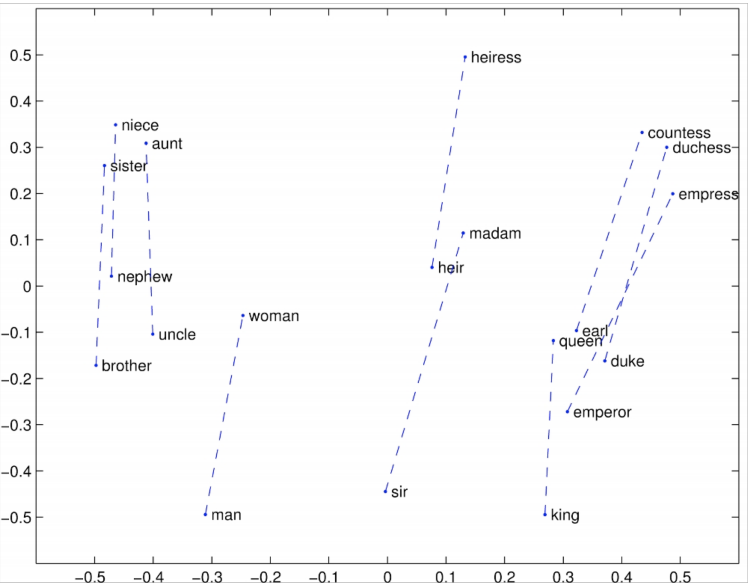
\includegraphics[width=0.5\textwidth]{images/glove_vecs.png}
%     \caption{GloVe words visualization in 2D space}
%     \label{fig:glove_ex}
% \end{figure}

These representations have a drawback that they fail to take context of a word into account. For example, the word \textit{`Scotland'} will have a different meaning in the sentence \textit{`Scotland is one of the most best places to live on earth'} than in the sentence \textit{`Royal Bank of Scotland is one of the top banking firms in the UK'}. The glove or word2vec word embedding will fail to differentiate the two meanings of Scotland and will assign same vector in both the cases. These drawbacks are tackled by a new concept of contextual word embeddings discussed in \cref{sec:context_we}

\subsubsection{Language Models}\label{sec:lm}

\begin{figure}
    \centering
    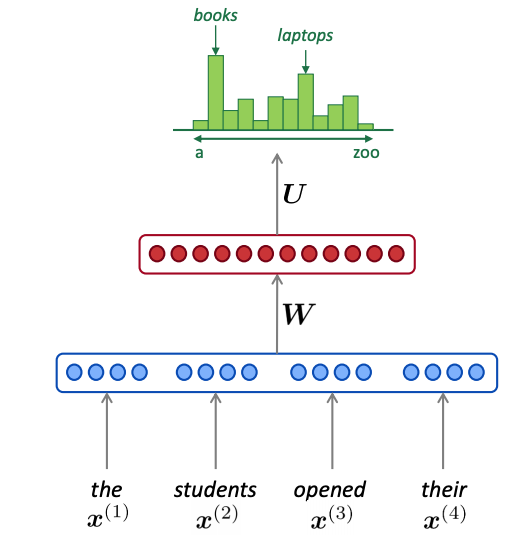
\includegraphics[width=0.45\textwidth]{images/lang_model.png}
    \caption{Prediction of next word using a Language Model}
    \label{fig:lang_model}
\end{figure}

A language model is a type of system that predicts the probability of possible next words given a sequence of words as the input. In general terms, for a given sequence of input $(x_{1}, x_{2}, \cdots, x_{t})$, the probability distribution of next term $x_{t+1}$ is computed from a vocabulary $V$ of $k$ words ($V = (w_{1}, w_{2}, \cdots, w_{k})$). 

\begin{equation}
    \label{eq:lm_dist}
        P(x_{t+1}|x_{1}, \cdots, x_{t})
\end{equation}

Earlier the language models were based on statistical approaches where they used to take a window of $n$ words as a context from the sentence to predict the next word. This approach is also known as $ngram$ Language Model. It takes an simple approach of calculating the conditional probability of next word in the sentence given the window of $n$ words as a context. These $ngram$ probabilities are calculated from counting them in some large corpus of text.

\begin{equation}
    \label{eq:lm_ngram}
        P(x_{t+1}|x_{1}, \cdots, x_{t}) = 
            \frac {P(x_{t+1}, x_{t}, \cdots, x_{t-n+2})} {P(x_{t}, \cdots, x_{t-n+2})}
\end{equation}

or in simpler terms:

\begin{equation}
    \label{eq:lm_count_ngram}
        P(w_{3}|w_{1},w_{2}) = \frac{count(w_{1}, w_{2}, w_{3})}{count(w_{1}, w_{2})}
\end{equation}

This statistical approach has mainly two problems. First sparsity, consider the \cref{eq:lm_count_ngram}, what if $w_{1}$, $w_{2}$ and $w_{3}$ never occurred together. The probability of $w_{3}$ will be 0. Also, if $w_{1}$ and $w_{2}$ then there's no way to calculate the probability of $w_{3}$. Second storage, as we increase the value of $n$, the count of all $nrgams$ we see in the corpus increases as well and so does the need of memory to store them.

The neural language model using Recurrent Neural Networks (\cref{sec:rnn}) were able to model all the words in a sentence without having a need of window to predict the next word at each timestep using hidden state and output from the previous time step combining with the new input at each time step. 


\subsubsection{Recurrent Neural Networks} \label{sec:rnn}
Text is a sequential form of data. To process text and extract information we need a model capable of processing the sequential data. \textit{Recurrent Neural Networks} \cite{elman1990finding} are the most elementary deep learning architectures that are able to learn from sequential data. RNN, are wide in nature as they unroll through time. These networks will have a `memory' component which can store the information about previous state. They share same set of weights throughout the layers, however, will receive a new input at every layer or time-step. The output to every time-step is dependent on the input taken at the current time-step $t_{i}$ as well as the information gained from previous time-step $t_{i-1}$. Specifically, an RN Net will maintain a hidden state $h_{t}$ at every step which is referred as the memory of network. An illustrated diagram of unrolled RNN is shown in fig \cref{fig:rnn_unrolled} \footnote{taken from \url{https://colah.github.io/posts/2015-08-Understanding-LSTMs/}}.

\begin{figure}
    \centering
    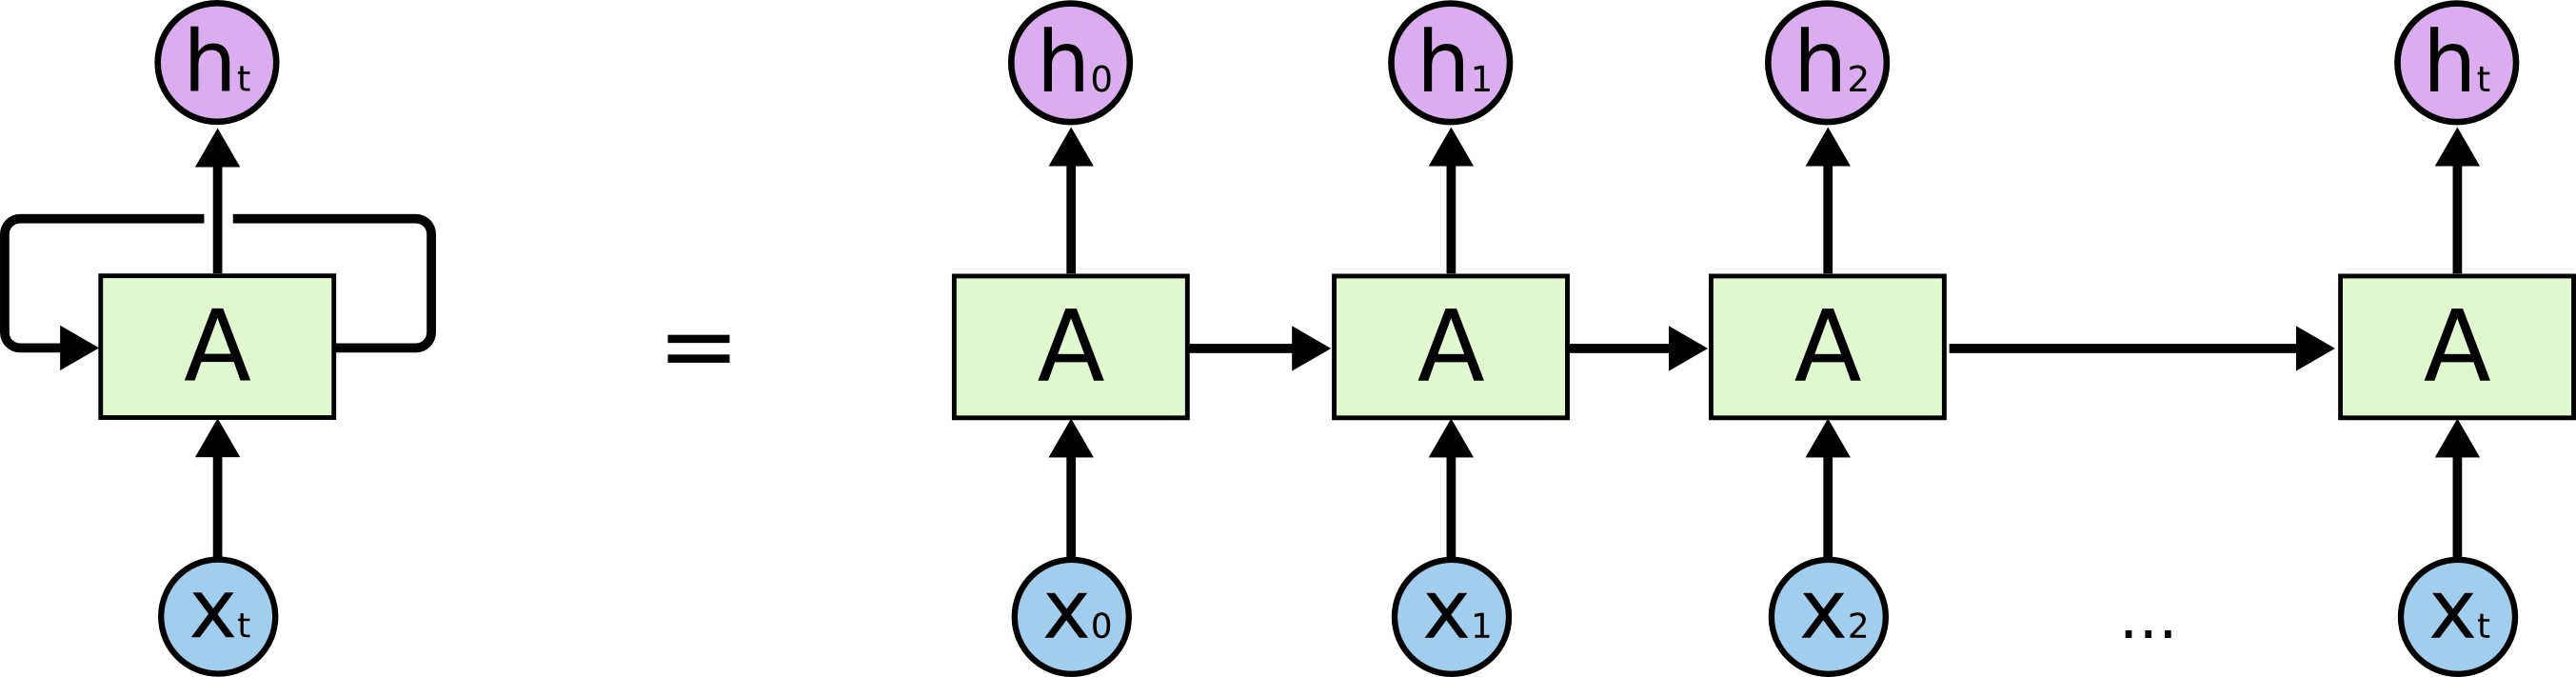
\includegraphics[width=\textwidth]{images/RNN-unrolled.png}
    \caption{RNN Unrolled}
    \label{fig:rnn_unrolled}
\end{figure}

The operations performed in RNN at every time step is given in the \cref{eq:rnn}.

\begin{align}\label{eq:rnn}
    \begin{gathered}
        h_{t} = \sigma_{h}(W_{e}x_{t} + W_{h}h_{t-1} + b_{h}) \\
        y_{t} = \sigma_{y}(W_{y}h_{t} + b_{y})
    \end{gathered}
\end{align}

Here $\sigma_{y}$ and $\sigma_{h}$ are the activation functions. $W_{h}$ is the weight matrix to apply transformation on previous hidden state $h_{t-1}$, $W_{e}$ is the weight matrix to apply transformation on the input $x_{t}$ received over time $t$. Combining these with the bias $b_{h}$ yields hidden state $h_t$ for time $t$. Applying activation on the $h_{t}$ with $W_{y}$ gives the output $y_t$ for every time-step $t$.


\subsubsection{Long Short-Term Memory Networks}
Although, in theory the RNNs are designed to handle the sequence input but in practice they lack in storing the long term dependencies because of the problem of exploding and vanishing gradients \cite{bengio1994learning}. Long Short-Term Memory Networks \cite{hochreiter1997long} are the advanced version of RNNs with a slight modification of being capable of deciding what to `remember' and what to `forget' from the input sequence with the help of a series of gates. LSTM has a number of gates, an output gate, an input gate $i_{t}$, forget gate $f_{t}$, $o_{t}$, all of which are the functions of previous hidden state $h_{t}$ and current input $x_{t}$. These gates interact with the previous cell state $c_{t-1}$, the current input $x_{t}$, and the current cell state $c_{t}$ and enable the model to selectively retain or information from the sequence. The full version of LSTM is given in the \cref{eq:lstm}.

\begin{equation}\label{eq:lstm}
    \begin{gathered}    
        f_{t} = \sigma_{g} (W_{f}x_{t} + U_{f}h_{t-1} + b_{f}) \\
        i_{t} = \sigma_{g} (W_{i}x_{t} + U_{i}h_{t-1} + b_{i}) \\
        o_{t} = \sigma_{g} (W_{o}x_{t} + U_{o}h_{t-1} + b_{o}) \\
        \Tilde{c_{t}} = \sigma_{c} (W_{c}x_{t} + U_{c}h_{t-1} + b_c)\\
        c_{t} = f_{t} \circ c_{t-1} + i_{t} \circ \Tilde{c_{t}}\\
        h_{t} = o_{t} \circ \sigma_{h}(c_{t})
    \end{gathered}
\end{equation}

where $\sigma_{g}$ is the $sigmoid$ activation function, $\sigma_{c}$ and $\sigma_{h}$ are the $tanh$ activation function, and $\circ$ is element-wise multiplication, also known as \textit{`Hadamard product'}. An illustrated diagram of unrolled RNN is shown in fig \cref{fig:lstm} \footnote{taken from \url{https://colah.github.io/posts/2015-08-Understanding-LSTMs/}}.

\begin{figure}
    \centering
    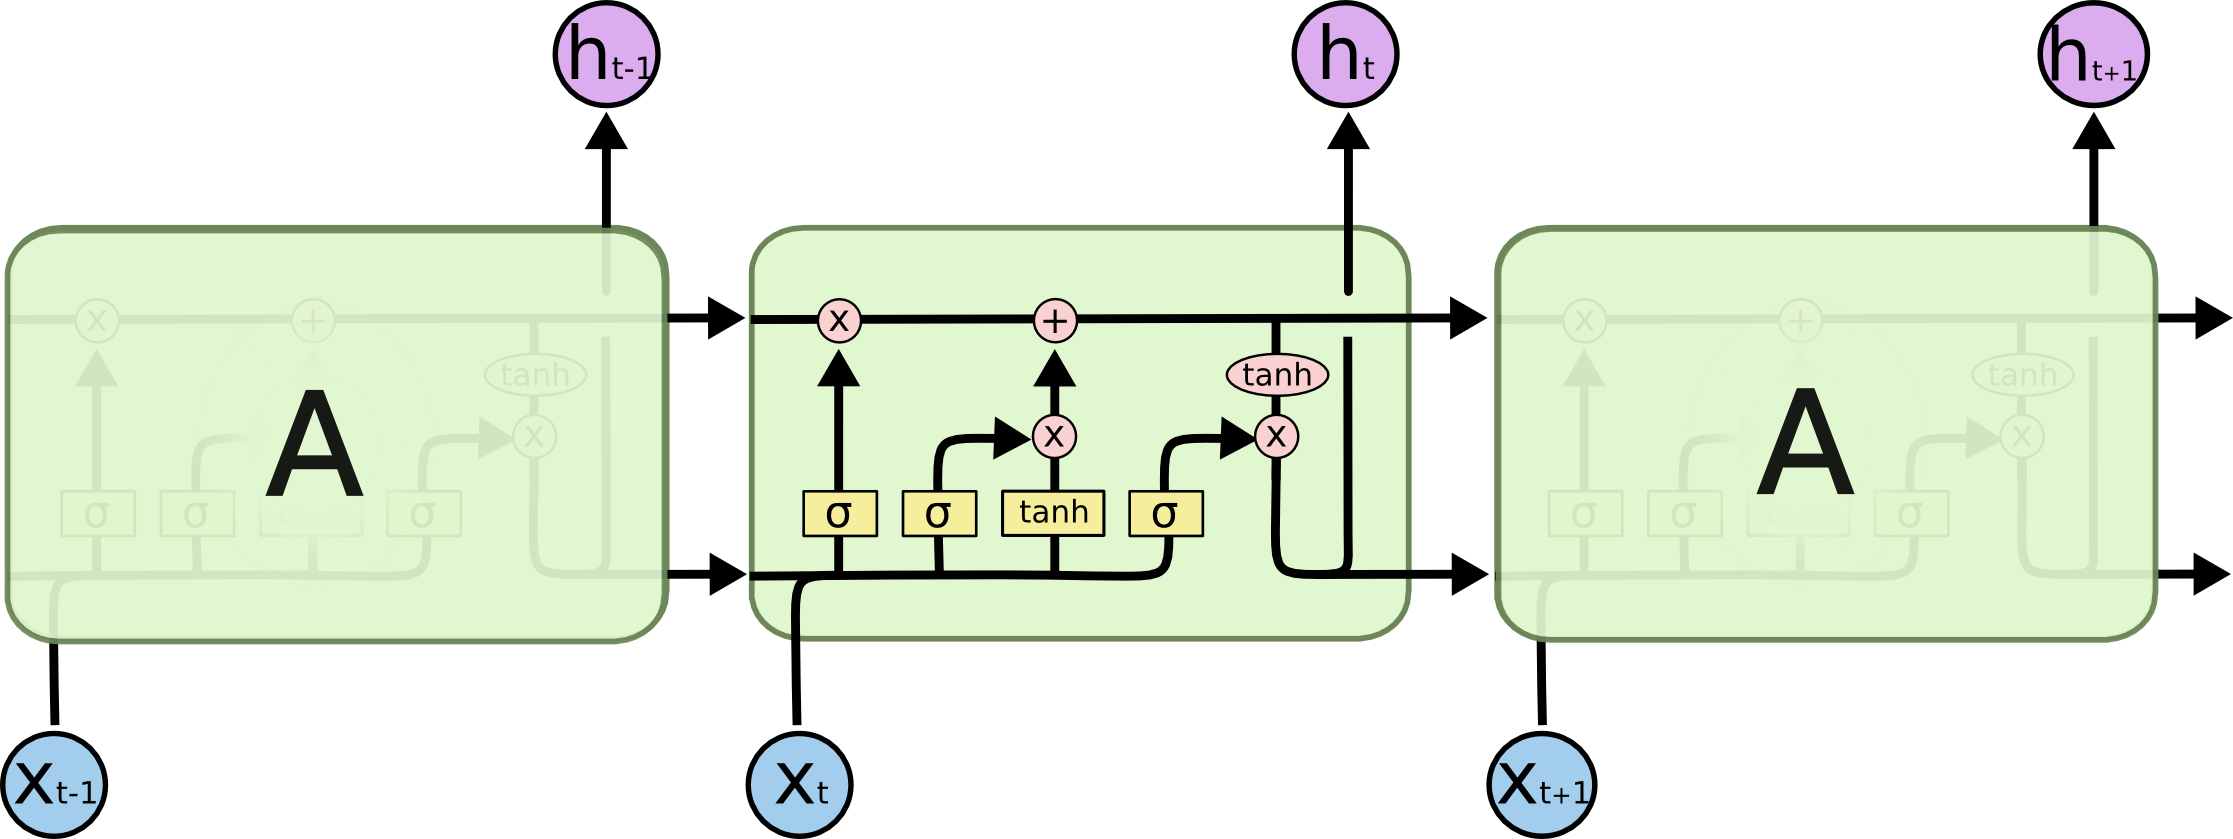
\includegraphics[width=\textwidth]{images/lstm.png}
    \caption{LSTM}
    \label{fig:lstm}
\end{figure}

LSTM layers can be stacked on each other to form multiple layer LSTM architecture. One of the most popular LSTM architecture is Bidirectional LSTM (BiLSTM) \cite{graves2013hybrid}, where two separate LSTMs are ran forward and backward to gain the sequential information in both directions.

\subsubsection{Convolutional Neural Networks}
Convolutional Neural Networks \cite{lecun1998gradient} are the version of deep neural networks established as state-of-the-art in various computer vision tasks \cite{barbu2019objectnet,ali2019mfc}. After the release of AlexNet \cite{krizhevsky2012imagenet} in ImageNet competition 2012, CNNs have been the benchmark for almost every vision task. Inspired from the popularity of CNN in vision, researchers proposed an CNN architecture for sentence classification which outperformed many benchmarks on various text classification dataset ranging from sentiment analysis to topic classification \cite{kim2014convolutional}. 

\begin{figure}
    \centering
    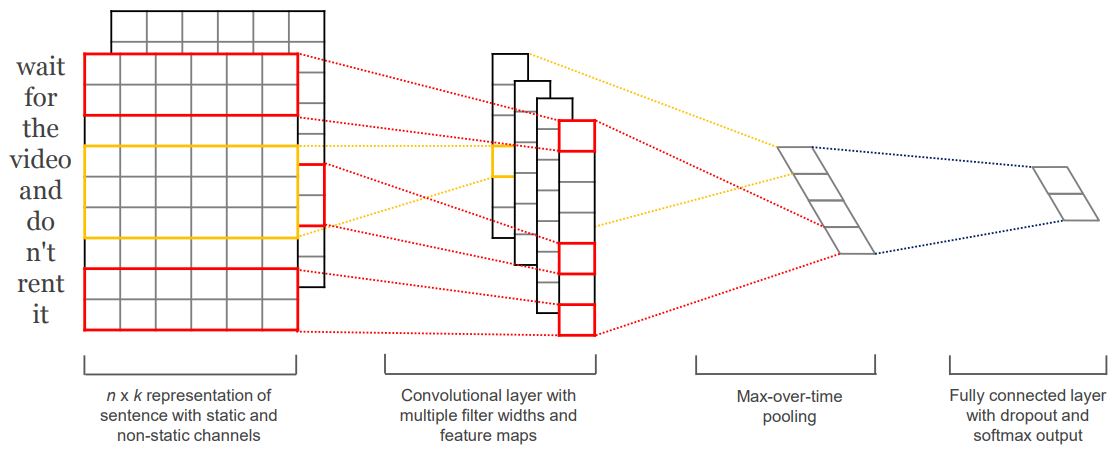
\includegraphics[width=\textwidth]{images/cnn_text.png}
    \caption{CNN for sentence classification}
    \label{fig:cnn}
\end{figure}

CNNs are capable of computing vectors for all possible sub-phrases in a sentence, not just grammatically correct one as done by RNNs. A CNN takes an input sentence of word length $n$ where each word is represented distributively in $d$ dimension. So the input $X_{1:n}$ is a $2D$ matrix of shape $n \times d$  where $x_{i}$ $\epsilon$ $\mathbb{R}^d$. Input $X_{1:n}$ can be represented as \cref{eq:cnn_input}.

\begin{equation}
    \label{eq:cnn_input}
    X_{1:n} = x_{1} \oplus x_{2} \oplus \cdots \oplus x_{n}
\end{equation}

where $\oplus$ is the concatenation operator. On the input layer, convolution filter $W$  $\epsilon$ $\mathbb{R}^{hd}$ is applied over window of $h$ words to generate a new feature. So, a feature $c_{i}$ is generated from the word window $x_{i:i+h-1}$ with the following operation:

\begin{equation}
    c_{i} = \sigma (Wx_{i:i+h-1} + b)
\end{equation}

where $W$ is the weight matrix for the connections, $\sigma$ is the activation function and $b$ $\epsilon$ $\mathbb{R}$ is the bias. Now, this filter is applied to each possible window of words giving an feature map $C$ $\epsilon$ $\mathbb{R}^{n-h+1}$.

\begin{equation}
    C = [c_{1}, c_{2}, \cdots, c_{n-h+1}]
\end{equation}

The entries in feature map $C$ are sharing the parameter $W$, where each $c_{i}$ $\epsilon$ $C$ is a result of calculation on small segment of the input. Then a $max-pooling$ operation is applied on these feature maps to capture the most important part.

\begin{equation}
    \Tilde{C} = max(C)
\end{equation}

This parameter sharing helps the model to incorporate an inductive bias into the model, helping to become learn the location invariant local features. There are $k$ number of filters applied to the input with different window sizes which are then concatenated to form a vector $\textbf{K}$ $\epsilon$ $\mathbb{R}^k$. Which is then fed to next hidden layer or output layer.

An illustrated diagram of an CNN architecture for text classification is shown in fig \cref{fig:cnn} \footnote{taken from \cite{kim2014convolutional}}.

\subsubsection{Sequence  to Sequence Models}
Most of the NLP tasks require sequential output instead of a single output label unlike classification or regression \cite{sutskever2014sequence}. These tasks can be Machine Translation of natural language, Question-Answering or Summary generation systems. These systems take a sequence of input and process it to produce yet another sequence for output. The goal is to take a sequence $(x_{1}, x_{2}, \cdots, x_{n})$ as input and map it to another sequence $(y_{1}, y_{2}, \cdots, y_{n})$ as output.

The architecture used to deal with these kind of problems is known as Sequence to Sequence model or in common terms, seq2seq model. It is a combination of auto-encoders and decoders which works in a sequential manner where encoder is an neural architecture to generate a context vector from input sequence and decoder, another neural architecture taking context vector as input and generating the output sequence.

The encoder takes an input $X$ and maps it to fixed size context vector $Z$ using the formula \cref{eq:enc}

\begin{equation}
    \label{eq:enc}
        Z = \sigma(WX + b)
\end{equation}

where $\sigma$ is activation function. A decoder then maps the context vector $Z$ to a new form of input $X^{\prime}$ as shown in equation \cref{eq:dec}

\begin{equation}
    \label{eq:dec}
        X^{\prime} = \sigma^{\prime}(W^{\prime}Z + b^{\prime})
\end{equation}

where $\sigma^{\prime}$ is another activation function. The loss is calculated as the squared error between original and reconstructed input as shown in equation \cref{eq:seq2seq_loss}. An illustrated diagram of seq2seq model is shown in fig \cref{fig:enc_dec} \footnote{Taken from \url{http://web.stanford.edu/class/cs224n/}}.

\begin{equation}
    \label{eq:seq2seq_loss}
        L = ||X-X^{\prime}||^{2}
\end{equation}

\begin{figure}
     \centering
     \begin{subfigure}[b]{0.25\textwidth}
         \centering
         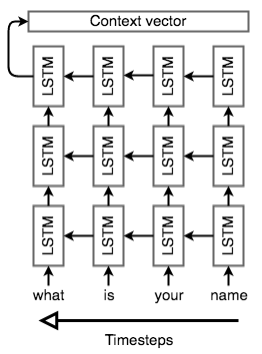
\includegraphics[width=\textwidth]{images/encoder.png}
         \caption{Encoder}
         \label{fig:encoder}
     \end{subfigure}
    %  \hfill
     \begin{subfigure}[b]{0.25\textwidth}
         \centering
         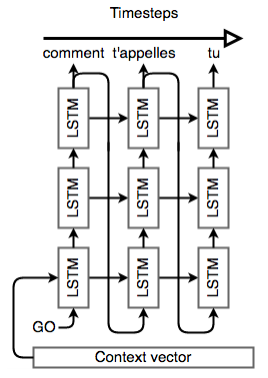
\includegraphics[width=\textwidth]{images/decoder.png}
         \caption{Decoder}
         \label{fig:decoder}
     \end{subfigure}
        \caption{Encoder-Decoder architecture using LSTM for seq2seq model}
        \label{fig:enc_dec}
\end{figure}

\paragraph{Attention} A problem with general encoder-decoder model is that they give equal importance to all the parts of input sequence. Also, the input sequence is compressed into a single context vector which creates the bottleneck problem, where a long information is tried to be kept into one small representation. 

A solution to this problem was proposed in the work \cite{bahdanau2014neural} introducing a new mechanism called Attention. Attention aligns the output at each decoding step to the whole input sequence in order to learn the most important part of the input aligning with the current step output by providing an attentive output.

Let's say we have calculated the encoding hidden states $(h_{1},  h_{2}, \cdots, h_{n})$ for the input sequence $(x_{1}, x_{2}, \cdots, x_{n})$ during the calculation of context vector $Z$. For a decoder hidden state $s_{t}$ on timestep $t$, we get attention score $e^{t}$ as follows:

\begin{equation}
    \label{eq:att_score}
        e^{t} = [s^{T}_{t}h_{1}, \cdots, s^{T}_{t}h_{n}]
\end{equation}

We take the softmax of these scores to get the attention distribution at timestep $t$.

\begin{equation}
    \label{eq:att_dist}
        \alpha^{t} = softmax(e^{t})
\end{equation}

The attention output $a_{t}$ is then calculated as the weighted sum of encoder hidden state using $\alpha^{t}$:

\begin{equation}
    \label{eq:att_out}
        a_{t} = \sum_{i=1}^{n} \alpha_{i}^{t}h_{i}
\end{equation}

Finally, we concatenate the attention output $a_{t}$ with decoder hidden state $s_{t}$ and proceed to calculate the negative log loss same as the non-attention decoder model.

\subsubsection{Contextual Word Embeddings}\label{sec:context_we}
As discussed in \cref{sec:word_emb}, the word embeddings generated by algorithms like word2vec \cite{mikolov2013distributed} and GloVe \cite{pennington2014glove} lacks the contextual awareness and fail to differentiate a word with different sense. For example, word $get$ has thirty different senses (meaning) in wordnet \footnote{\url{https://wordnet.princeton.edu/}} based on the different contexts. But if we use pre-trained word embeddings to generate the vector representation of $get$, it will be same for all the thirty times and we will loose the semantic information. 

A new trend of transfer learning came in Deep Learning based NLP with the introduction works like ELMo \cite{peters2018deep} and ULMFiT \cite{howard2018universal} where language models are used to learn the nuances of the language grammar and then the pre-trained language model is then fine-tuned on a task specific dataset to achieve better results.

\begin{figure}
    \centering
    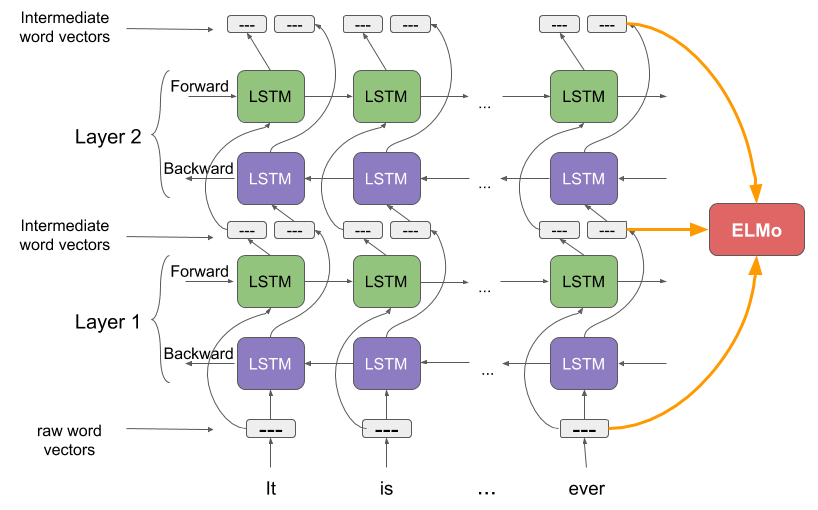
\includegraphics[width=0.75\textwidth]{images/elmo.png}
    \caption{ELMo Vector Representation}
    \label{fig:elmo}
\end{figure}

\paragraph{ELMo} stands for Embeddings Learned from Language Models \cite{peters2018deep} uses a bidirectional language model to capture the context of a word in a sentence from both sides (left to right and vice-versa). ELMo uses an character-level CNN to convert raw text into a word vector which is then fed into a bidirectional language model. The ouput of this BiLM is then sent to the next layer of BiLM to form a set of intermediate word vectors. The final output of ELMo is the weighted sum of raw vectors and the intermediate vectors formed from two layers of the BiLMs. The two language models used here are based on LSTM architectures. An illustration of ELMo is shown is \cref{fig:elmo} \footnote{Taken from \url{https://www.analyticsvidhya.com/blog/2019/03/learn-to-use-elmo-to-extract-features-from-text/}}.

ELMo achieved 9\% error reduction on the SQuAD (question-answering) dataset compared to then state-of-the-art, 16\% on Ontonotes SRL dataset, 10\% on Ontonotes coreference dataset and 4\% on CoNLL 2003 dataset. It paved a huge path in the success of contextualized word representations for different tasks in NLP.

\paragraph{ULMFiT} stands for Universal Language Model Fine Tuning, introduced the way of applying transfer learning on text classification problem \cite{howard2018universal}. It does so in three main steps: first, train an general domain language model on large corpus of text (mainly Wikipedia); second, fine tune the language model on task specific target dataset; and third, use the again fine tune the fine-tuned language model as classifier by adding a softmax activation on top with target dataset. An illustration of the three steps of ULMFiT is shown in \cref{fig:ulmfit_steps}.

% \begin{figure}
%     \centering
%     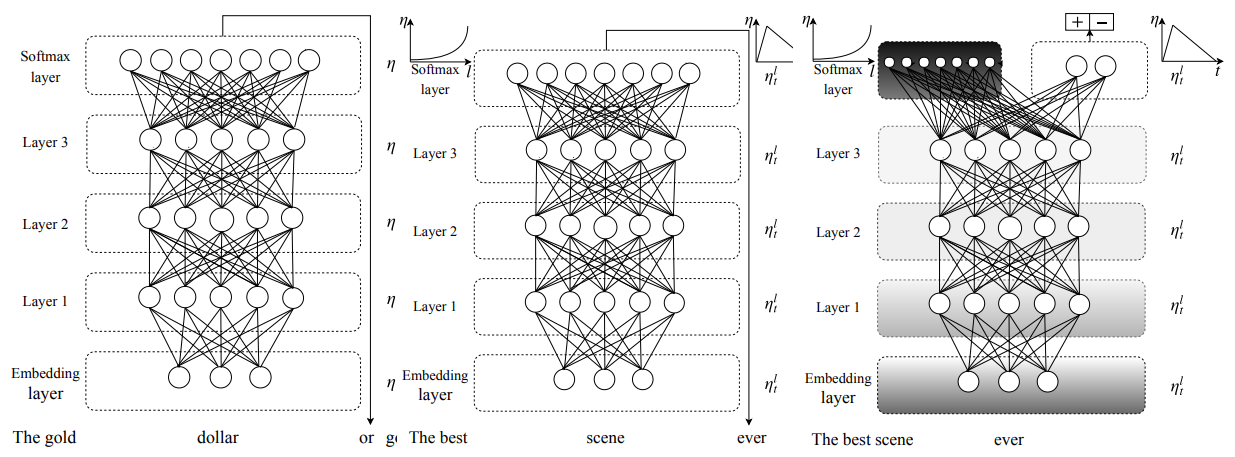
\includegraphics[width=\textwidth]{images/ulmfit.png}
%     \caption{ULMFiT Steps}
%     \label{fig:ulmfit}
% \end{figure}

\begin{figure}
     \centering
     \begin{subfigure}[b]{0.3\textwidth}
         \centering
         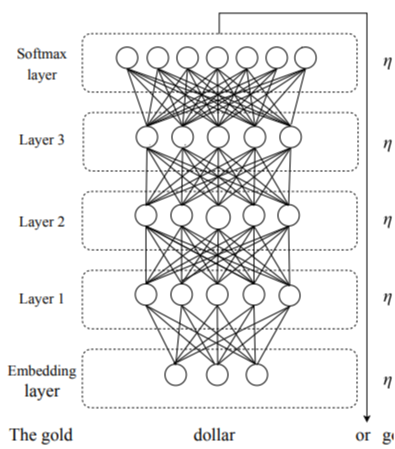
\includegraphics[width=\textwidth]{images/ulm1.png}
         \caption{LM Training}
         \label{fig:lm_train}
     \end{subfigure}
    %  \hfill
     \begin{subfigure}[b]{0.3\textwidth}
         \centering
         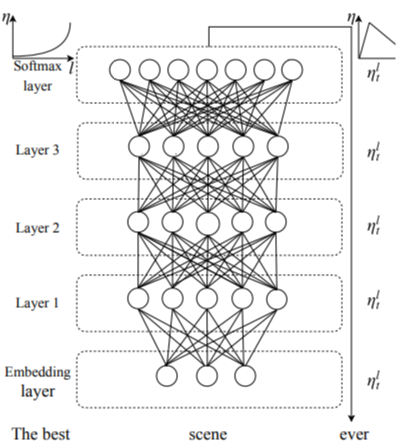
\includegraphics[width=\textwidth]{images/ulm2.png}
         \caption{LM Fine-Tuning}
         \label{fig:lm_ft}
     \end{subfigure}
    %  \hfill
     \begin{subfigure}[b]{0.3\textwidth}
         \centering
         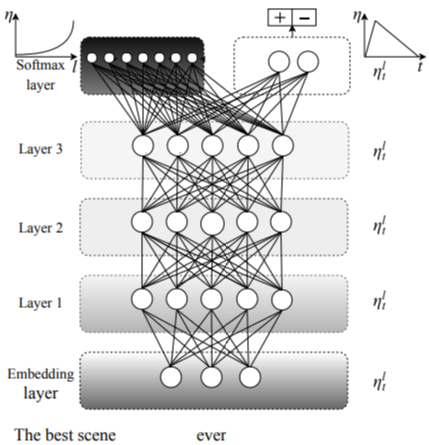
\includegraphics[width=\textwidth]{images/ulm3.png}
         \caption{Classifier Training}
         \label{fig:lm_classif}
     \end{subfigure}
        \caption{ULMFiT Steps \cite{howard2018universal}}
        \label{fig:ulmfit_steps}
\end{figure}


ULMFiT achieved better results for text classification on six different datasets ranging from topic classification to sentiment analysis. It did so by learning the general rules of grammar from huge corpus of text and then transferring that learning with fine tuning on a task-specific dataset providing better results than state-of-the-arts \cite{howard2018universal}.

\subsubsection{Transformers}\label{sec:transformers}
Almost all of the models we discussed have recurrent behaviour, which can not be trained parallely. This imposes a huge problem of time taken to train a model from scratch. In the work \cite{vaswani2017attention}, authors proposed a new neural architecture called Transformers which uses a combination of self attention and feed-forward network in its encoder-decoder model and doesn't require any recurrent or convolutional elements. This new seq2seq model was a huge success where it gained better performance on various sequential NLP tasks. To name one, it improved the machine translation performance by 10\% on WMT EN-FR and WMT EN-DE datasets. It also reduced the training time by large margin benefiting its non-recurrent nature \cite{vaswani2017attention}.

The success of transformer architecture paved the way for development of new models to solve the sequential tasks. It helped NLP researchers to utilize its non-recurrent nature in transfer learning where the transformer is used for general pre-training of a language model on large corpus of text which can be used for fine-tuning on domain specific dataset for downstream tasks. An encoder-decoder model of Transformer architecture is shown in the \cref{fig:trans}.

\begin{figure}
    \centering
    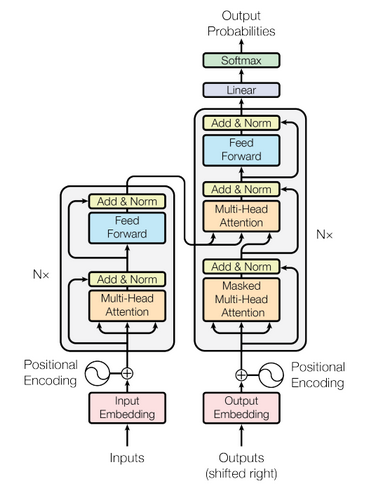
\includegraphics[width=0.5\textwidth]{images/transformer.png}
    \caption{Transformer architecture \cite{vaswani2017attention}.}
    \label{fig:trans}
\end{figure}

\paragraph{Generative Pre-Training}
One of the earliest works in using Transformers for pre-training of language model was presented in \cite{radford2018improving}. Following the idea from ELMo \cite{peters2018deep}, authors proposed a language model using transformer decoder trained on large corpus and then fine-tuned on task specific dataset. The main difference of GPT from ELMo is that ELMo uses two independent LSTM language models to caputre the forwards and backward context whereas in case of GPT, it uses a uni-directional multi-layer transformer language model capable of capturing context due to its attentive nature.

ELMo takes a feature based approach of feeding feature vectors for different tasks into different models, whereas GPT takes a fine-tuning based approach where same language model trained on huge corpus is fine-tuned for downstream tasks without changing the architecture. An illustration of a GPT model used for pre-training is shown in \cref{fig:gpt} \footnote{Taken from \url{https://openai.com/blog/language-unsupervised/}}.

\begin{figure}
    \centering
    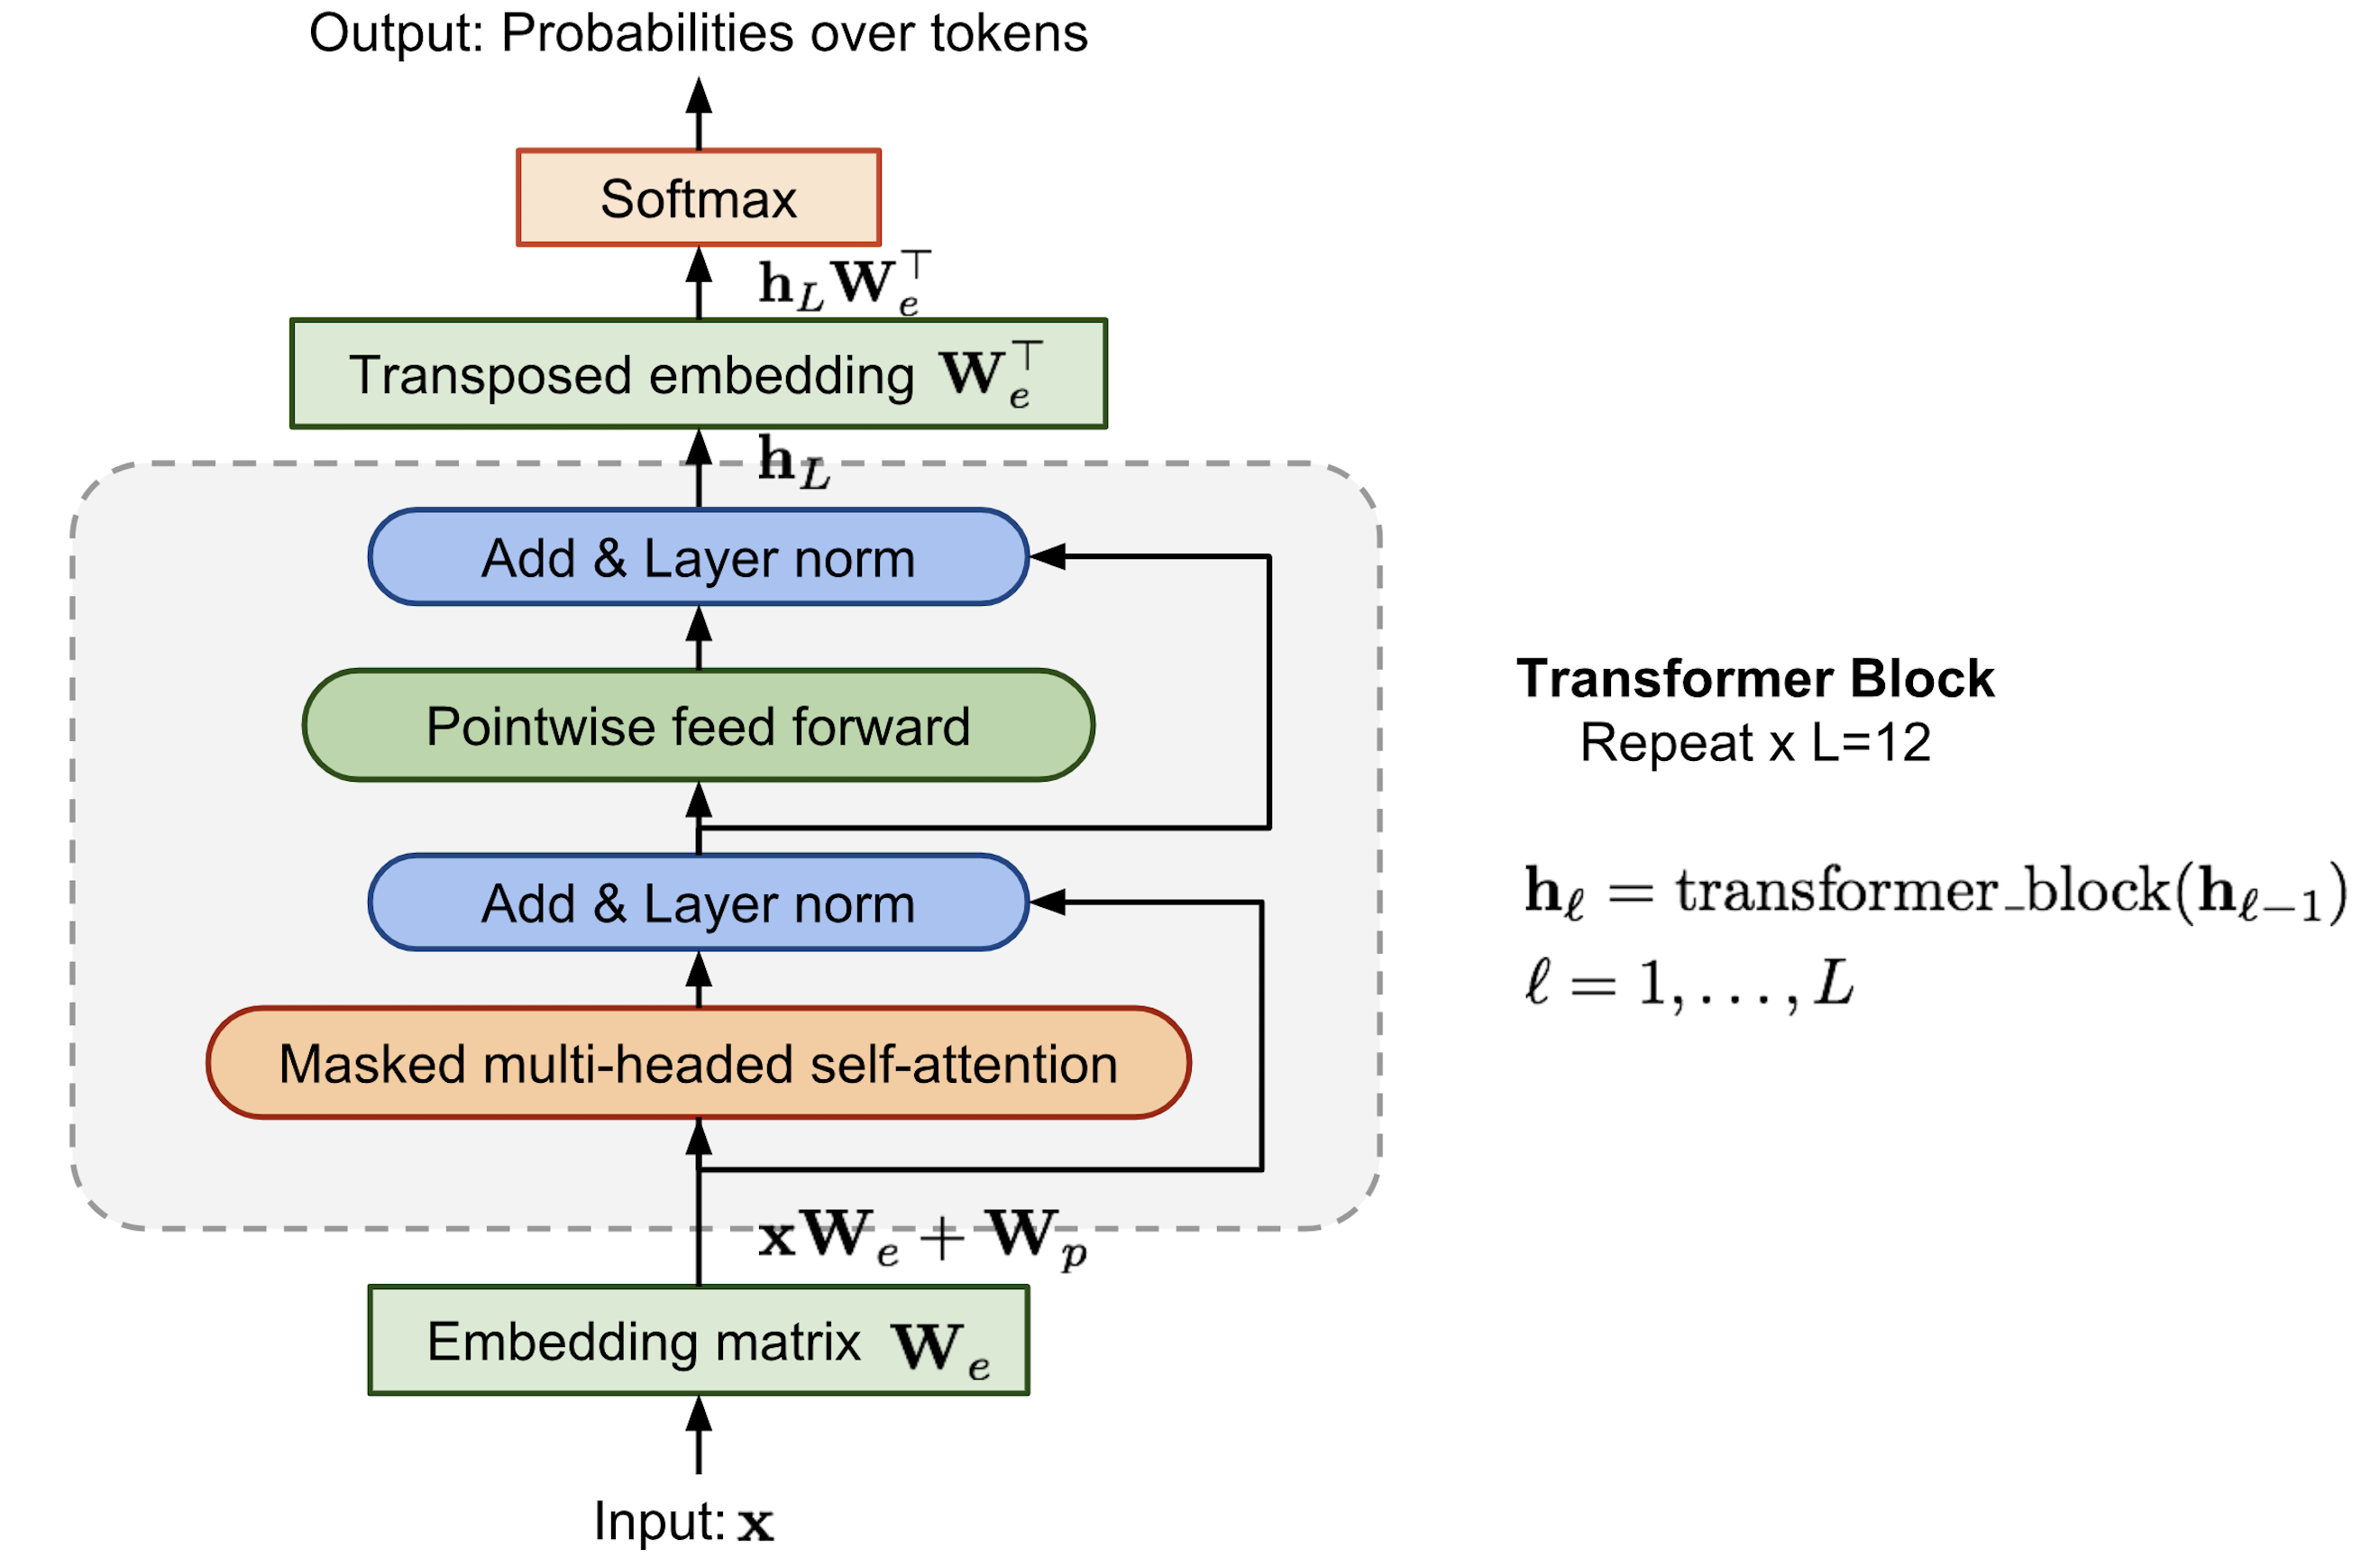
\includegraphics[width=0.75\textwidth]{images/GPT.png}
    \caption{GPT architecture.}
    \label{fig:gpt}
\end{figure}

\paragraph{Bidirectional Encoder Representation from Transformers}
BERT \cite{devlin2018bert} is another example of the success of transfer learning in NLP. BERT is a bidirectional transformer language model trained on a large text corpus that can be fine-tuned on any domain specific dataset for the downstream tasks like text classification or named entity recognition. BERT mainly differs from other models like GPT and ELMo because of the pre-training tasks used during the unsupervised training of language model. It involves two tasks; first, Masked Language Model (MLM) \cite{taylor1953cloze} or prediction of the masked word in a sentence, and second, prediction of next sentence from the corpora.

For the first task of Masked Language Model, let’s say we have a sentence ‘Boris Johnson is the Prime Minister of UK’. So instead of training for prediction of next word in the sentence as a general Language Model, BERT pre-training replaces 15\% of the words with a [MASK] token and learns to predict the correct word at the position of [MASK] token. In the second task of Next Sentence Prediction, the model is trained to learn the relationship between sentences where for a given sentence pair A \& B, the model is asked to predict if the sentence B is actually the next sentence that comes after A or not?

BERT improved the fine-tuning based approach of GPT by using a bidirectional transformer for masked language modelling by learning the both left and right context which is a huge improved over GPT's unidirectional approach specially for token-level tasks like Question Answering where the answer depends on both left and right contexts. An illustrated diagram of BERT pre-training and fine-tuning is shown in \cref{fig:bert1}. 
% A visual comparison between BERT, GPT and ELMo architectures presented in the work \cite{devlin2018bert} is shown in \cref{fig:bert2}.

\begin{figure}
    \centering
    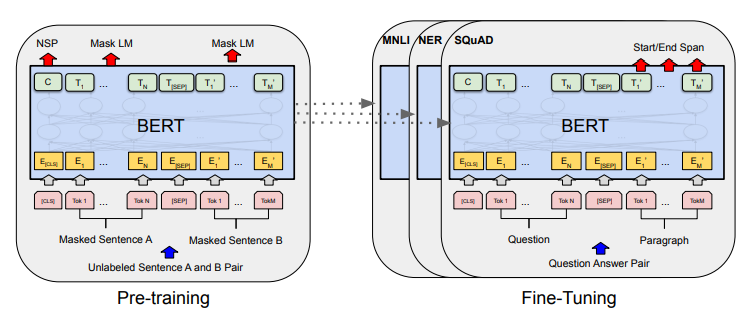
\includegraphics[width=0.75\textwidth]{images/bert1.png}
    \caption{BERT \cite{devlin2018bert}}
    \label{fig:bert1}
\end{figure}


% \begin{figure}
%     \centering
%     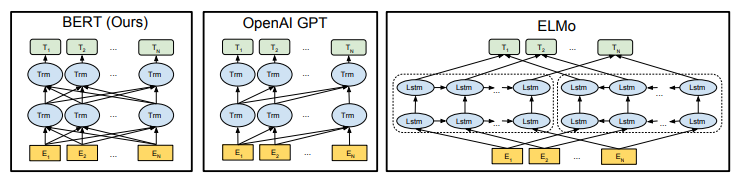
\includegraphics[width=\textwidth]{images/bert2.png}
%     \caption{BERT, GPT and ELMo \cite{devlin2018bert}}
%     \label{fig:bert2}
% \end{figure}


% \subsection{Current State-of-the-Art}\label{sec:sotas}
In the literature, current State-of-the-Arts (SOTA) for almost all of the NLP tasks are based on deep learning learning algorithms. In the \cref{tab:sotas} we will list few works and their performance on the tasks defined in \cref{sec:tasks}.

\begin{sidewaystable}[!htbp]
  \begin{center}
    \caption{Current State-of-the-Arts. We can see that almost all of the works are based on deep learning.}
    \label{tab:sotas}
    \begin{tabular}{|c|c|c|c|c|}
      \hline
      \textbf{Task} & \textbf{Work} & \textbf{Model} & \textbf{Performance} & \textbf{Data}\\
      \hline
      \textbf{NER} & \cite{baevski2019cloze} & CNN Large + fine-tune & 93.5 F1 & CoNLL 2003\\
      & \cite{strakova-etal-2019-neural} & LSTM-CRF+ELMo+BERT+Flair & 93.38 F1 & CoNLL 2003\\
      \hline
      \textbf{POS Tagging} & \cite{Bohnet_2018} & Meta BiLSTM & 97.96 Acc & Penn Treebank\\
      & \cite{Heinzerling_2019} & Multilingual BERT and BPEmb & 96.77 Acc &  Universal Dependencies\\
      \hline
      \textbf{NLI} & \cite{liu2019roberta} & RoBERTa & 90.8 Acc & Multi-NLI\\
      & \cite{yang2019xlnet} & XLNet-Large & 90.2 Acc & Multi-NLI\\
      \hline
      \textbf{Relation Extraction} & \cite{lai-etal-2018-sunnynlp} & SVM with GloVe & 0.76 F1 & SemEval 2018 Task 10\\
      & \cite{baldini-soares-etal-2019-matching} & BERT: Matching-the-Blanks & 89.5 F1 & SemEval 2010 Task 8\\
    %   \hline
    %   SRL & \cite{he-etal-2018-jointly} & ELMo Modified & 85.5 & OntoNotes\\
    %   & \cite{peters2018deep} & ELMo & 84.6 & OntoNotes\\
    %   \hline
    %   Dependency Parsing & 25.113231 & d &   & Penn Treebank\\
    %   & 1110.1 & a &   & Universal Dependencies\\
      \hline
      \textbf{Machine Translation} & \cite{edunov2018understanding} & Transformer Big & 35 BLEU  & WMT 2014 EN-DE\\
      & \cite{edunov2018understanding} & Transformer Big & 45.6 & WMT 2014 EN-FR\\
    %   \hline
    %   Data Augmentation & 25.113231 & d &   & imdb\\
    %   & 1110.1 & a &   & Amazon Reviews\\
    %   \hline
    %   Summary Generation & 25.113231 & d &   & CNN/Daily Mail\\
    %   & 1110.1 & a &   & CNN/Daily Mail\\
      \hline
      \textbf{Question Answering} & \cite{lan2019albert} & ALBERT (ensemble model) & 92.21 F1 & SQuAD\\
      & \cite{lan2019albert} & ALBERT (single model) & 90.9 F1 & SQuAD\\
      \hline
      \textbf{Text Classification} & \cite{yang2019xlnet} & XLNet & 0.62 Error & Dbpedia\\ 
      & \cite{yang2019xlnet} & XLNet & 4.49 Error & AG News\\
    %   \hline
    %   Aspect-Based Sentiment & 25.113231 & d &   & SemEval-2014 Task 4\\
    %   & 1110.1 & a &   & SemEval-2014 Task 4\\
      \hline
    \end{tabular}
  \end{center}
\end{sidewaystable}

% \subsection{Business Process}\label{business_process}
% % \label{sec:use_in_business}
% \paragraph{Cold Start \& Concept Drift} We have seen from the \cref{tab:sotas} that deep learning has given better results with ample amount of data available for training. But the problem in a business process is with the availability of data itself. Deep learning can provide better performance but will require a huge amount of resource to train the models. 

% In a business process it is hard to get ample amount of data in the initial phase and hence we face the problem of cold start. We need to train our models with less data only, which results in reduced performance. Also, in a business process we keep receiving data as time goes on like stream of data. After some times, we may get new data that might be enough to train a deep learning model. And there is high chance that the relationship between problem and solution changes as well. Hence it is important to address the problem of concept drift as well.

% Less Data

% Class Imbalance

% But deep learning has its own consequences, and that is the resource needed for the training of a deep learning model. It takes a lot of labelled data for training a deep learning model, as well as the training itself takes a long time and very powerful system to run the process on. Even if we can out-source the training process to cloud services like AWS or Azure, we may reduce our expenses on time and machine but still we will need a lot of training data that should be labelled.

% These can be solved with methods like One shot learning or data augmentation to increase the training set. GANs

% With a general semi-supervised training on big corpus, the learning can be transferred to some domain specific task with minimal fine tuning for particular task.

% \subsection{Concept Drift}
% In industry, collecting a training data brings a new form of challenge: the challenge of concept drift. The problem is that during the start of a business process 
